
% ♥♥♥♥	♥♥♥♥
Les VBOs (Vertex Buffer Object) en OpenGL est une méthode qui permet d'envoyer des données vers la carte graphique, elle remplace les VA (Vertex Array) déclarés comme obsolètes par OpenGL qui étaient enregistrés sur le CPU et devaient transiter entre CPU et GPU.\\
Les VBOs ont été conçus afin d'optenir les meilleurs performances possibles. Son utilisation est actuellement la méthode la plus efficace en OpenGL car les données 3D ne résident plus dans la mémoire système mais dans la mémoire de la carte graphique ce qui permet un rendu plus rapide.\\
Les VAOs (Vertex Array Object) servent à optimiser l'utilisation des VBOs, ils sont une fonctionnalité toute nouvelle qui ressemble fortement aux Display Lists. Les VAOs permettent la "sauvegarde" de plusieurs commandes dans un seul et même objet qui lui même sera stocké dans la mémoire de la carte graphique. \\
Par exemple : ces commandes ou appels de fonctions peuvent utiliser des VBOs. Ainsi tout sera stocké directement dans la carte graphique et celle-ci n'aura plus à demander à l'application ce qu'elle doit faire. OpenGL pourra ainsi optimiser ses actions du faite qu'il connetra ses actions futurs. Ceci permet d'éviter de faire transiter trop d'informations entre le système et la carte graphique.
\subsection{Application d'un VA}
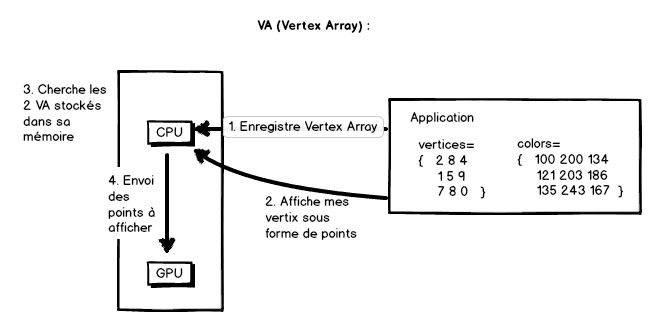
\includegraphics[width=10cm,height=5cm]{img/VA.png}
\subsection{Application d'un VBO}
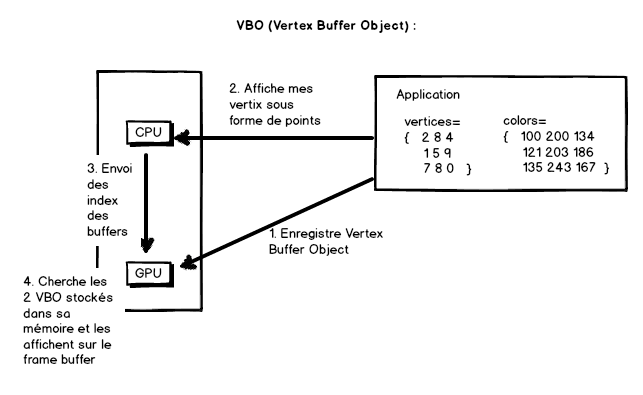
\includegraphics[width=10cm,height=5cm]{img/VBO.png}
\subsection{Application d'un VBO dans un VAO}
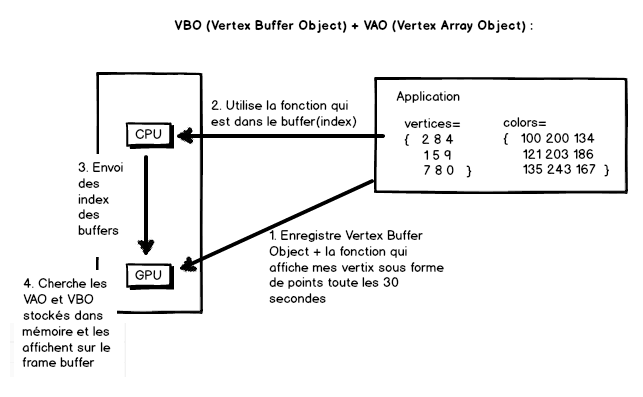
\includegraphics[width=10cm,height=5cm]{img/VAO_VBO.png}
%♥♥♥♥	♥♥♥♥